\documentclass{article}

%%%% packages and definitions (optional)
\usepackage{graphicx} % allows inclusion of graphics
\usepackage{graphics}
\usepackage{booktabs} % nice rules (thick lines) for tables
\usepackage{microtype} % improves typography for PDF
\usepackage[hidelinks]{hyperref}

\newcommand{\SN}{S$_N$}
\renewcommand{\vec}[1]{\bm{#1}} %vector is bold italic
\newcommand{\vd}{\bm{\cdot}} % slightly bold vector dot
\newcommand{\grad}{\vec{\nabla}} % gradient
\newcommand{\ud}{\mathop{}\!\mathrm{d}} % upright derivative symbol
\graphicspath{ {images/} }
\usepackage[affil-it]{authblk}
\usepackage{tikz}
\usetikzlibrary{positioning, arrows, decorations, shapes }



\usepackage[acronym,toc]{glossaries}
%\newacronym{<++>}{<++>}{<++>}
\newacronym[longplural={metric tons of heavy metal}]{MTHM}{MTHM}{metric ton of heavy metal}
\newacronym{ABM}{ABM}{agent-based modeling}
\newacronym{ACDIS}{ACDIS}{Program in Arms Control \& Domestic and International Security}
\newacronym{AHTR}{AHTR}{Advanced High Temperature Reactor}
\newacronym{ANDRA}{ANDRA}{Agence Nationale pour la gestion des D\'echets RAdioactifs, the French National Agency for Radioactive Waste Management}
\newacronym{ANL}{ANL}{Argonne National Laboratory}
\newacronym{ANS}{ANS}{American Nuclear Society}
\newacronym{API}{API}{application programming interface}
\newacronym{ARE}{ARE}{Aircraft Reactor Experiment}
\newacronym{ARFC}{ARFC}{Advanced Reactors and Fuel Cycles}
\newacronym{ASME}{ASME}{American Society of Mechanical Engineers}
\newacronym{ATWS}{ATWS}{Anticipated Transient Without Scram}
\newacronym{BDBE}{BDBE}{Beyond Design Basis Event}
\newacronym{BIDS}{BIDS}{Berkeley Institute for Data Science}
\newacronym{CAFCA}{CAFCA}{ Code for Advanced Fuel Cycles Assessment }
\newacronym{CDTN}{CDTN}{Centro de Desenvolvimento da Tecnologia Nuclear}
\newacronym{CEA}{CEA}{Commissariat \`a l'\'Energie Atomique et aux \'Energies Alternatives}
\newacronym{CI}{CI}{continuous integration}
\newacronym{CNEN}{CNEN}{Comiss\~{a}o Nacional de Energia Nuclear}
\newacronym{CNERG}{CNERG}{Computational Nuclear Engineering Research Group}
\newacronym{COSI}{COSI}{Commelini-Sicard}
\newacronym{COTS}{COTS}{commercial, off-the-shelf}
\newacronym{CSNF}{CSNF}{commercial spent nuclear fuel}
\newacronym{CTAH}{CTAHs}{Coiled Tube Air Heaters}
\newacronym{CUBIT}{CUBIT}{CUBIT Geometry and Mesh Generation Toolkit}
\newacronym{CURIE}{CURIE}{Centralized Used Fuel Resource for Information Exchange}
\newacronym{DAG}{DAG}{directed acyclic graph}
\newacronym{DANESS}{DANESS}{Dynamic Analysis of Nuclear Energy System Strategies}
\newacronym{DBE}{DBE}{Design Basis Event}
\newacronym{DESAE}{DESAE}{Dynamic Analysis of Nuclear Energy Systems Strategies}
\newacronym{DHS}{DHS}{Department of Homeland Security}
\newacronym{DOE}{DOE}{Department of Energy}
\newacronym{DRACS}{DRACS}{Direct Reactor Auxiliary Cooling System}
\newacronym{DRE}{DRE}{dynamic resource exchange}
\newacronym{DSNF}{DSNF}{DOE spent nuclear fuel}
\newacronym{DYMOND}{DYMOND}{Dynamic Model of Nuclear Development }
\newacronym{EBS}{EBS}{Engineered Barrier System}
\newacronym{EDF}{EDF}{Électricité de France}
\newacronym{EDZ}{EDZ}{Excavation Disturbed Zone}
\newacronym{EIA}{EIA}{U.S. Energy Information Administration}
\newacronym{EPA}{EPA}{Environmental Protection Agency}
\newacronym{EP}{EP}{Engineering Physics}
\newacronym{FCO}{FCO}{Fuel Cycle Options}
\newacronym{FCT}{FCT}{Fuel Cycle Technology}
\newacronym{FEHM}{FEHM}{Finite Element Heat and Mass Transfer}
\newacronym{FEPs}{FEPs}{Features, Events, and Processes}
\newacronym{FHR}{FHR}{Fluoride-Salt-Cooled High-Temperature Reactor}
\newacronym{FLiBe}{FLiBe}{Fluoride-Lithium-Beryllium}
\newacronym{GDSE}{GDSE}{Generic Disposal System Environment}
\newacronym{GDSM}{GDSM}{Generic Disposal System Model}
\newacronym{GENIUSv1}{GENIUSv1}{Global Evaluation of Nuclear Infrastructure Utilization Scenarios, Version 1}
\newacronym{GENIUSv2}{GENIUSv2}{Global Evaluation of Nuclear Infrastructure Utilization Scenarios, Version 2}
\newacronym{GENIUS}{GENIUS}{Global Evaluation of Nuclear Infrastructure Utilization Scenarios}
\newacronym{GPAM}{GPAM}{Generic Performance Assessment Model}
\newacronym{GRSAC}{GRSAC}{Graphite Reactor Severe Accident Code}
\newacronym{GUI}{GUI}{graphical user interface}
\newacronym{HLW}{HLW}{high level waste}
\newacronym{HPC}{HPC}{high-performance computing}
\newacronym{HTC}{HTC}{high-throughput computing}
\newacronym{HTGR}{HTGR}{High Temperature Gas-Cooled Reactor}
\newacronym{IAEA}{IAEA}{International Atomic Energy Agency}
\newacronym{IEMA}{IEMA}{Illinois Emergency Mangament Agency}
\newacronym{IHLRWM}{IHLRWM}{International High Level Radioactive Waste Management}
\newacronym{INL}{INL}{Idaho National Laboratory}
\newacronym{IPRR1}{IRP-R1}{Instituto de Pesquisas Radioativas Reator 1}
\newacronym{IRP}{IRP}{Integrated Research Project}
\newacronym{ISFSI}{ISFSI}{Independent Spent Fuel Storage Installation}
\newacronym{ISRG}{ISRG}{Independent Student Research Group}
\newacronym{JFNK}{JFNK}{Jacobian-Free Newton Krylov}
\newacronym{LANL}{LANL}{Los Alamos National Laboratory}
\newacronym{LBNL}{LBNL}{Lawrence Berkeley National Laboratory}
\newacronym{LCOE}{LCOE}{levelized cost of electricity}
\newacronym{LDRD}{LDRD}{laboratory directed research and development}
\newacronym{LFR}{LFR}{Lead-Cooled Fast Reactor}
\newacronym{LLNL}{LLNL}{Lawrence Livermore National Laboratory}
\newacronym{LMFBR}{LMFBR}{Liquid Metal Fast Breeder Reactor}
\newacronym{LOFC}{LOFC}{Loss of Forced Cooling}
\newacronym{LOHS}{LOHS}{Loss of Heat Sink}
\newacronym{LOLA}{LOLA}{Loss of Large Area}
\newacronym{LP}{LP}{linear program}
\newacronym{LWR}{LWR}{Light Water Reactor}
\newacronym{MA}{MA}{minor actinide}
\newacronym{MAGNOX}{MAGNOX}{Magnesium Alloy Graphie Moderated Gas Cooled Uranium Oxide Reactor}
\newacronym{MCNP}{MCNP}{Monte Carlo N-Particle code}
\newacronym{MILP}{MILP}{mixed-integer linear program}
\newacronym{MIT}{MIT}{the Massachusetts Institute of Technology}
\newacronym{MOAB}{MOAB}{Mesh-Oriented datABase}
\newacronym{MOOSE}{MOOSE}{Multiphysics Object-Oriented Simulation Environment}
\newacronym{MOX}{MOX}{mixed oxide}
\newacronym{MSBR}{MSBR}{Molten Salt Breeder Reactor}
\newacronym{MSRE}{MSRE}{Molten Salt Reactor Experiment}
\newacronym{MSR}{MSR}{Molten Salt Reactor}
\newacronym{NAGRA}{NAGRA}{National Cooperative for the Disposal of Radioactive Waste}
\newacronym{NEAMS}{NEAMS}{Nuclear Engineering Advanced Modeling and Simulation}
\newacronym{NEUP}{NEUP}{Nuclear Energy University Programs}
\newacronym{NFCSim}{NFCSim}{Nuclear Fuel Cycle Simulator}
\newacronym{NGNP}{NGNP}{Next Generation Nuclear Plant}
\newacronym{NMWPC}{NMWPC}{Nuclear MW Per Capita}
\newacronym{NNSA}{NNSA}{National Nuclear Security Administration}
\newacronym{NPRE}{NPRE}{Department of Nuclear, Plasma, and Radiological Engineering}
\newacronym{NQA1}{NQA-1}{Nuclear Quality Assurance - 1}
\newacronym{NRC}{NRC}{Nuclear Regulatory Commission}
\newacronym{NSF}{NSF}{National Science Foundation}
\newacronym{NSSC}{NSSC}{Nuclear Science and Security Consortium}
\newacronym{NUWASTE}{NUWASTE}{Nuclear Waste Assessment System for Technical Evaluation}
\newacronym{NWF}{NWF}{Nuclear Waste Fund}
\newacronym{NWTRB}{NWTRB}{Nuclear Waste Technical Review Board}
\newacronym{OCRWM}{OCRWM}{Office of Civilian Radioactive Waste Management}
\newacronym{ORION}{ORION}{ORION}
\newacronym{ORNL}{ORNL}{Oak Ridge National Laboratory}
\newacronym{PARCS}{PARCS}{Purdue Advanced Reactor Core Simulator}
\newacronym{PBAHTR}{PB-AHTR}{Pebble Bed Advanced High Temperature Reactor}
\newacronym{PBFHR}{PB-FHR}{Pebble-Bed Fluoride-Salt-Cooled High-Temperature Reactor}
\newacronym{PEI}{PEI}{Peak Environmental Impact}
\newacronym{PH}{PRONGHORN}{PRONGHORN}
\newacronym{PRIS}{PRIS}{Power Reactor Information System}
\newacronym{PRKE}{PRKE}{Point Reactor Kinetics Equations}
\newacronym{PSPG}{PSPG}{Pressure-Stabilizing/Petrov-Galerkin}
\newacronym{PWAR}{PWAR}{Pratt and Whitney Aircraft Reactor}
\newacronym{PWR}{PWR}{Pressurized Water Reactor}
\newacronym{PyNE}{PyNE}{Python toolkit for Nuclear Engineering}
\newacronym{PyRK}{PyRK}{Python for Reactor Kinetics}
\newacronym{QA}{QA}{quality assurance}
\newacronym{RDD}{RD\&D}{Research Development and Demonstration}
\newacronym{RD}{R\&D}{Research and Development}
\newacronym{RELAP}{RELAP}{Reactor Excursion and Leak Analysis Program}
\newacronym{RIA}{RIA}{Reactivity Insertion Accident}
\newacronym{RIF}{RIF}{Region-Institution-Facility}
\newacronym{SFR}{SFR}{Sodium-Cooled Fast Reactor}
\newacronym{SINDAG}{SINDA{\textbackslash}G}{Systems Improved Numerical Differencing Analyzer $\backslash$ Gaski}
\newacronym{SKB}{SKB}{Svensk K\"{a}rnbr\"{a}nslehantering AB}
\newacronym{SNF}{SNF}{spent nuclear fuel}
\newacronym{SNL}{SNL}{Sandia National Laboratory}
\newacronym{STC}{STC}{specific temperature change}
\newacronym{SUPG}{SUPG}{Streamline-Upwind/Petrov-Galerkin}
\newacronym{SWF}{SWF}{Separations and Waste Forms}
\newacronym{SWU}{SWU}{Separative Work Unit}
\newacronym{TRIGA}{TRIGA}{Training Research Isotope General Atomic}
\newacronym{TRISO}{TRISO}{Tristructural Isotropic}
\newacronym{TSM}{TSM}{Total System Model}
\newacronym{TSPA}{TSPA}{Total System Performance Assessment for the Yucca Mountain License Application}
\newacronym{ThOX}{ThOX}{thorium oxide}
\newacronym{UFD}{UFD}{Used Fuel Disposition}
\newacronym{UML}{UML}{Unified Modeling Language}
\newacronym{UOX}{UOX}{uranium oxide}
\newacronym{UQ}{UQ}{uncertainty quantification}
\newacronym{US}{US}{United States}
\newacronym{UW}{UW}{University of Wisconsin}
\newacronym{VISION}{VISION}{the Verifiable Fuel Cycle Simulation Model}
\newacronym{VV}{V\&V}{verification and validation}
\newacronym{VVER}{VVER}{Voda-Vodyanoi Energetichesky Reaktor (Russian Pressurized Water Reactor)}
\newacronym{WIPP}{WIPP}{Waste Isolation Pilot Plant}
\newacronym{YMR}{YMR}{Yucca Mountain Repository Site}

	
\makeglossaries

\title{Future Nuclear Inventory Analysis of the European Union with CYCLUS, an Agent-Based Fuel Cycle Simulator.}
\author{Jin Whan Bae, Kathyrn Huff, Clifford Singer}
\affil{Dept. of Nuclear, Plasma, and Radiological Engineering, University of Illinois at Urbana-Champaign
	
		  Urbana, IL}
\date{}                     %% if you don't need date to appear
\setcounter{Maxaffil}{0}
\renewcommand\Affilfont{\itshape\small}
%%%%%%%%%%%%%%actual words%%%%%%%%%%%%%%%%%%%%%%%%%%%%%%%%%%%%%%%%%%%%%%%%%%%%5


\begin{document}
\maketitle
	
\section{Abstract}
Numerous nuclear fuel cycle system modeling codes
have been developed to perform fuel cycle transition
analyses from a once-through cycle to an advanced
fuel cycle. Verification studies compare different
fuel cycle analysis tools against each other to
test agreement and identify sources of difference.
This paper benchmarks \Cyclus, the agent-based,
open-source fuel cycle simulation code, against
a verification study \cite{feng_standardized_2016} with
DYMOND \cite{yacout_modeling_2005},
VISION \cite{jacobson_verifiable_2010},
ORION \cite{gregg_analysis_2012}, and
MARKAL \cite{shay_epa_2006}. The study reveals
that \Cyclus' results match the spreadsheet results
very closely, with minor differences caused by
reactor module behavior.

\section{Introduction}
Fuel cycle simulators act as an important tool to
aid decision in policy and fuel cycle strategies.
To meet this need from various institutions, a
multitude of fuel cycle simulators were developed,
using different methods and different structures
to simulate the material flow in the nuclear fuel cycle.
The difference in the algorithm of fuel cycle analysis
codes combined with a small user community make
validation studies necessary to gain
confidence of the capability of the code as well as its
agreement with other analysis codes.

This study is done to benchmark \Cyclus' results
against that of other well-known codes, such as
DYMOND \cite{yacout_modeling_2005},
VISION \cite{jacobson_verifiable_2010},
ORION \cite{gregg_analysis_2012}, and
MARKAL \cite{shay_epa_2006}. We take the input
parameters and results from a validation study
\cite{feng_standardized_2016} already done for the
mentioned tools for a transition scenario from an
open fuel cycle to an advanced fuel cycle with
reprocessing. In the paper, the `model solutions'
generated from an excel worksheet are compared
with each code results, and the results show
excellent agreement.


\subsection{\Cyclus}

\Cyclus is an agent-based fuel cycle simulation framework 
\cite{huff_fundamental_2016}, which means 
that each reactor, reprocessing plant, and fuel fabrication plant is modeled as an agent.
A \Cyclus simulation contains prototypes, which are fuel cycle facilities with
pre-defined parameters, that are deployed in the simulation as \texttt{facility} agents.
Encapsulating the \texttt{facility} agents are the \texttt{Institution} and \texttt{Region}.
A \texttt{Region} agent holds a set of \texttt{Institution}s.
An \texttt{Institution} agent can deploy or decommission \texttt{facility} agents.
The \texttt{Institution} agent is part of a \texttt{Region} agent,
which can contain multiple \texttt{Institution} agents. Several versions of \texttt{Institution}
and \texttt{Region} exist, varying in complexity and functions \cite{huff_extensions_2014}.
 \texttt{DeployInst} is used as the institution archetype for this work, where the institution
deploys agents at user-defined timesteps.

At each timestep (one month),
agents make requests for materials or bid to supply them and exchange
with one another. A market-like mechanism called the dynamic resource exchange
\cite{gidden_agent-based_2015} governs the exchanges.
Each material resource has a quantity, composition, name, and a unique identifier
for output analysis. The timestep execution in \Cyclus follows 
\texttt{Build, Tick, \gls{DRE}, Tock, and Decommission}, as illustrated in
figure \ref{fig:time}. The \texttt{Tick}, and \texttt{Tock} phases are for
each agent to perform actions, such as transmutation, separation, generation,
of materials before and after the market exchange phase. 

\begin{figure}[h]
\centering
\scalebox{0.7}{
\begin{tikzpicture}[node distance=1.5cm]
\node (Build) [process] {Build (kernel)};
\node (Tick) [process, below of=Build] {Tick (agent)};
\node (DRE) [process, below of=Tick]{Dynamic Resource Exchange (kernel) };
\node (Tock) [process, below of=DRE]{Tock (agent)};
\node (Decom) [process, below of=Tock] {Decommission (kernel)};

\draw [arrow] (Build) -- (Tick); 
\draw [arrow] (Tick) -- (DRE);
\draw [arrow] (DRE) -- (Tock);
\draw [arrow] (Tock) -- (Decom);
\end{tikzpicture}
}
\caption{\Cyclus timestep execution steps.}
\label{fig:time}
\end{figure}

The modularity of \Cyclus allows a low barrier of
entry for developers, since developers can create an
archetype (e.g. Reactor module, Reprocessing module)
without extensive knowledge of the \Cyclus framework.

\section{Scenario Specifications}

\subsection{Historical Operation of EU Reactors}
\begin{itemize}
	\item \textbf{Simulation Time:}  1970-2050 
	\item \textbf{Reprocessing Capacity:}  91.6 MTHM per month \cite{schneider_spent_2008}  
	\item \textbf{Reprocessing Efficiency:}  99.8\%  
	\item \textbf{Reprocessing Streams:}  Plutonium and Uranium  
	\item \textbf{\gls{MOX} Fabrication:}  ~10\% Reprocessed Pu and ~90\% Depleted Uranium  
	\item \textbf{\gls{MOX} Fabrication Throughput}: 30 MTHM per month per facility \cite{hugelmann_melox_1999}
	\item \textbf{\gls{MOX} Fuel Reprocessing Stage:}  Infinite - used \gls{MOX} fuel gets reprocessed again.  
	\item\textbf{Reprocessed Uranium Usage:}  None. Stockpile reprocessed Uranium. \\
\end{itemize} 

\subsection{French Transition to \gls{SFR}}
\begin{itemize}
	\item \textbf{Simulation Time:}  1970-2160
	\item \textbf{Reprocessing Capacity:}  infinite 
	\item \textbf{Reprocessing Efficiency:}  99.8\%  
	\item \textbf{Reprocessing Streams:} Plutonium and Uranium
	\item \textbf{Initial Spent \gls{UOX} and Depleted Uranium inventory}: Mass from first simulation - none is added.
	\item \textbf{No Continued Source of Spent \gls{UOX} or Depleted Uranium}  
	\item \textbf{\gls{MOX} Fabrication:}  ~10\% Reprocessed Pu and ~90\% Depleted Uranium  
	\item \textbf{\gls{MOX} Fabrication Throughput}: infinite
	\item \textbf{\gls{MOX} Fuel Reprocessing Stage:}  Infinite - used \gls{MOX} fuel gets reprocessed again.  
	\item\textbf{Reprocessed Uranium Usage:}  None. Stockpile reprocessed Uranium. \\
\end{itemize}

\section{Reactor Specifications}



\begin{table}[h]
	\centering
	\label{tab:pwr}
	\begin{tabular}{|c|c|}
		\hline
		Specification & Value \\
		\hline
		PWR Cycle Time & 18 months \\ 
		PWR Refueling Outage & 2 months \\
		Fuel Mass per Assembly & 523.4 kg \\
		Num. of Aseem. per Core & 257 for 1,330 MWe, linearly adjusted\\
		Num. of Assem. per Batch & 1/3 of the core \\
		Fuel & French \glspl{PWR} prefer \gls{MOX} but also accept \gls{UOX}\\
		\hline
	\end{tabular}
	\caption {\gls{PWR} Specifications}
	\end{table}
	
\begin{table}[h]
	\centering
	\label{tab:sfr}
	\begin{tabular}{|c|c|}
		\hline
		Specification & Value \\
		\hline
		SFR Cycle Time & 12 months \\ 
		SFR Refueling Outage & 2 months \\
		Fuel Mass per Batch & 16,300 kg \\
		Batch per Core & 4 \\
		Power Output & 600 MWe \\
		Fuel & \gls{MOX}\\
		\hline
	\end{tabular}
	\caption {\gls{SFR} ASTRID Specifications}
	\cite{marsault-marie-sophie_pre-conceptual_2012}
\end{table}


\section{Current Status}
The current status of the EU reactors can be identified easily
in an \gls{IAEA} \gls{PRIS} database \cite{IAEA_PRIS_2017}.
The acquired csv file from \gls{PRIS} is then used to create a
Cyclus input file, and is run.


\section{Future Nuclear Projections}

The future of nuclear energy in EU nations is organized
in the table by the World Nuclear Association \cite{world_nuclear_association_nuclear_2017}.
All the planned constructions are completed in their expected date without delay
or failure. Also, the newly constructed nuclear power plants are assumed to have a lifetime of 60 years.

Table \ref{tab:eu_deployment} lists the reactors that are currently under construction or planned.

 
\begin{table}[h]
	\centering
	\caption {Power Reactors under construction and planned \cite{world_nuclear_association_nuclear_2017}}
	\label{tab:eu_deployment}
	\scalebox{0.70}{
	\begin{tabular}{|c|c|c|c|c|}
		\hline
		Exp. Operational & Country & Reactor & Type & Gross MWe\\
		\hline
		2018 & Slovakia  & Mochovce 3 & PWR & 440\\
		2018 & Slovakia & Mochovce 4 & PWR & 440 \\
		2018 & France & Flamanville 3 & PWR & 1600 \\
		2018 & Finland & Olkilouto 3 & PWR & 1720 \\		
		2019 & Romania & Cernavoda 3 & PHWR & 720 \\
		2020 & Romania & Cernavoda 4 & PHWR & 720 \\
		2024 & Finland & Hanhikivi & VVER1200 & 1200 \\
		2024 & Hungary & Paks 5 & VVER1200 & 1200 \\
		2025 & Hungary & Paks 6 & VVER1200 & 1200 \\
		2025 & Bulgaria & Kozloduy 7 & AP1000? & 950 \\
		2026 & UK & Hinkley Point C1 & EPR & 1670 \\
		2027 & UK & Hinkley Point C2 & EPR & 1670 \\
		2029 & Poland & Choczewo? & N/A & 3000 \\
		2035 & Poland & East? & N/A & 3000 \\
		2035 & Czech Rep & Dukovany 5 & ? & 1200 \\
		2035 & Czech Rep & Temelin 3 & AP1000? & 1200 \\
		2040 & Czech Rep & Temelin 4 & AP1000? & 1200 \\
		\hline
	\end{tabular}
	}
\end{table}


For each EU nation, the growth trajectory is categorized from
"Aggressive Growth" to "Aggressive Shutdown". Aggressive growth is
characterized by a rigorous expansion of nuclear power while 
Aggressive Shutdown is characterized as a transition to rapidly
de-nuclearize the nation's electric grid. A nation's growth trajectory is
categorized into five categories:

\begin{itemize}
	\item Aggressive Growth
	\item Modest Growth 
	\item Maintenance
	\item Modest Reduction
	\item Aggressive Reduction
\end{itemize}

The growth trajectory and specific plan of each nation in the EU 
is listed in Table \ref{tab:eu_growth}.

\begin{table}[h]
	\centering
	\label{tab:eu_growth}
		\begin{tabular}{|c|c|c|}
			\hline
			Nation & Growth Trajectory & Specific Plan \\
			\hline
			France & Modest Reduction & Shutdown nuclear plants if they reach end of lifetime. No new construction.\\
			Germany & Aggressive Reduction & Close all nuclear reactors by 2022.\\
			Czech Republic & Modest Growth & Additional 2,400 MWe (AP1000s) by 2035.\\
			UK & Aggressive Growth & 13 units (17,900 MWe) by 2030.\\
			Belgium & Aggressive Reduction & All shutdown 2025.\\
			Sweden & Aggressive Reduction & All shutdown 2050.\\
			Finland & Modest Growth & Additional EPR in 2018, VVER in 2024.\\
			Bulgaria & Modest Growth & Additional AP1000 (1,000 MWe) construction in 2035. \\
			Poland & Aggressive Growth & Additional 6,000 MWe by 2035.\\
			Romania & Modest Growth & Additional 1,440 MWe by 2020. \\
			Hungary & Modest Growth & Additional 2,400 MWe (VVER-1200) by 2025. \\ 
			Spain & Maintenance & No plans to expand or early shutdown. \\
			Italy & Maintenance  & No plans to expand or early shutdown. \\
			\hline
		\end{tabular}
	\caption {Future Nuclear Programs of EU Nations \cite{world_nuclear_association_nuclear_2017}}
\end{table}


\section{Results}

Each \Cyclus result is shown as a solid line, and the excel solution in the
paper is shown as a dotted line, for better visualization. The results are
simply a reproduction of the plots displayed in the paper. The excel
results are obtained by personal contact with the paper author
Bo Feng at Argonne National Laboratory.

Most results from \Cyclus show excellent agreement. Differences in results
stem from the errors associated with averaging and the concept of what
constitutes a `snapshot' of a facility inventory.

The deployed reactor capacity is shown in figure \ref{fig:pow_plot}.
The \gls{LWR} retirement and \gls{SFR} deployment timeseries are shown
in figure \ref{fig:dep}. The two plots show exact agreement with the
excel solutions from the paper.

\begin{figure}[htbp!]
	\begin{center}
		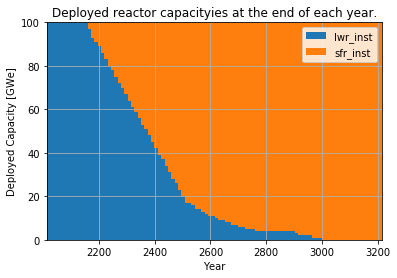
\includegraphics[scale=0.6]{./images/results_18/power_plot.png}
	\end{center}
        \caption{Deployed reactor capacities at the end of each year.}
	\label{fig:pow_plot}
\end{figure}



\begin{figure}[htbp!]
	\begin{center}
		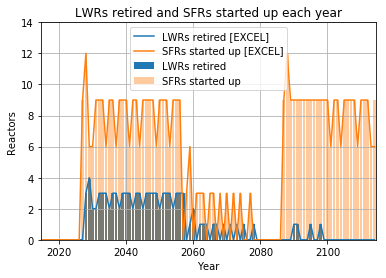
\includegraphics[scale=0.6]{./images/results_18/dep.png}
	\end{center}
        \caption{\glspl{LWR} retired and \glspl{SFR} started up each year.}
	\label{fig:dep}
\end{figure}


The annual fuel loading rates are shown in table \ref{fig:fuel_load}.
The initial fuel loading for 100 \gls{LWR} reactors were edited to match
the plot in the verification
study results. Note the oscillations for the \gls{LWR} fuel loading
is caused by the refueling period being 18-month refuel cycle for all \gls{LWR} reactors
aggregated into 12-month groups. Note also that the total values
are equal for both plots.

Although indistinguishable,
there is a small difference with \gls{SFR} fuel loading, that is proportional
to the core mass difference, as mentioned in the previous section.
Figure \ref{fig:fuel_load_diff_norm} shows the
differences normalized by the core mass differences, overlapped with the
\gls{SFR} deployment. This is to show that the differences only occur during
deployment due to the difference in core mass.


\begin{figure}[htbp!]
    \begin{center}
        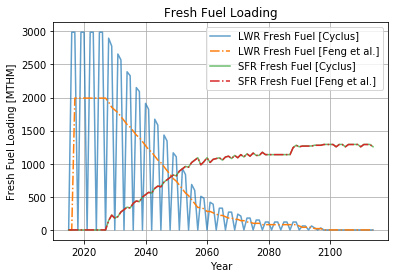
\includegraphics[scale=0.6]{./images/results_18/fuel_load.png}
    \end{center}
        \caption{Annual fresh fuel loading rates (first cores and reload fuel).}
    \label{fig:fuel_load}
\end{figure}


\begin{figure}[htbp!]
    \begin{center}
        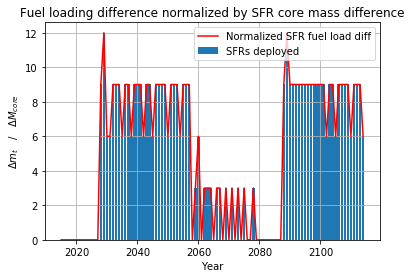
\includegraphics[scale=0.6]{./images/results_18/fuel_load_diff_norm.png}
    \end{center}
        \caption{Difference of annual fresh fuel loading rates (Cyclus - Excel) normalized by the core mass difference of an \gls{SFR} due to fractional batch size.}
    \label{fig:fuel_load_diff_norm}
\end{figure}


The inventory of discharged \gls{UNF} in mandatory cooling stage is shown
in figure \ref{fig:fuel_discharge}. It also oscillates between the excel solution,
and converges. This is due to the annual averaging of
the \gls{UNF} inventory. For a better visual, the monthly inventory is shown
in figure \ref{fig:fuel_discharge_monthly}, where the oscillation is more obvious.
Note that for most plots the \gls{SFR} inventory and fuel loading is almost
exactly the same as the excel solutions, minus the small difference due to core
size.

\begin{figure}[htbp!]
    \begin{center}
        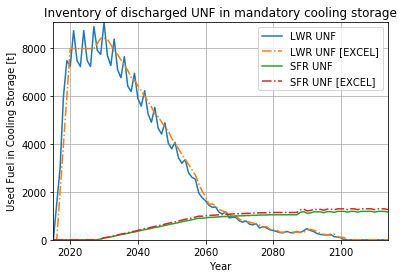
\includegraphics[scale=0.6]{./images/results_18/fuel_discharge.png}
    \end{center}
        \caption{Inventory of discharged \gls{UNF} in mandatory cooling storage.}
    \label{fig:fuel_discharge}
\end{figure}


\begin{figure}[htbp!]
    \begin{center}
        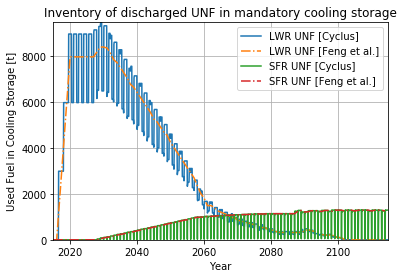
\includegraphics[scale=0.6]{./images/results_18/fuel_discharge_monthly.png}
    \end{center}
        \caption{Inventory of discharged \gls{UNF} in mandatory cooling storage.}
    \label{fig:fuel_discharge_monthly}
\end{figure}


Similar results are shown in figure \ref{fig:waiting} for the inventory of discharge fuel cooled and waiting
for reprocessing. Non-aggregated monthly values are shown in figure \ref{fig:waiting_monthly}.
However, note that the oscillation peaks meet with the excel
solution.  This is because cooled inventory is measured by the cumulative sum
of fuel that has been cooled minus the fuel reprocessed at that timestep.
The cooled inventory before the fuel are sent to reprocessing, which correspond
to the peaks in the oscillation, are the cooled inventory defined by the paper.

\begin{figure}[htbp!]
    \begin{center}
        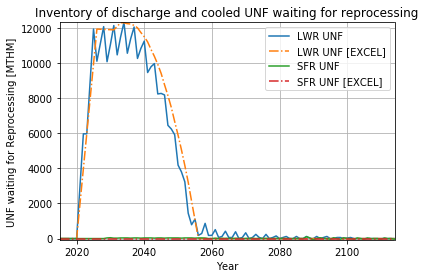
\includegraphics[scale=0.6]{./images/results_18/waiting.png}
    \end{center}
        \caption{Inventory of discharged and cooled \gls{UNF} waiting for reprocessing}
    \label{fig:waiting}
\end{figure}

\begin{figure}[htbp!]
    \begin{center}
        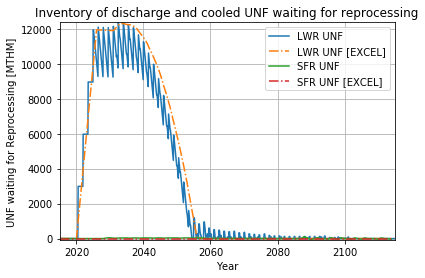
\includegraphics[scale=0.6]{./images/results_18/waiting_monthly.png}
    \end{center}
        \caption{Inventory of discharged and cooled \gls{UNF} waiting for reprocessing.}
    \label{fig:waiting_monthly}
\end{figure}


Figure \ref{fig:rep} shows the reprocessing throughput, which also oscillates between
the excel solution. Note that there is no oscillation in the beginning because the
\gls{LWR} reprocessing plant throughput is maximized at 2,000 tons per year. 

\begin{figure}[htbp!]
    \begin{center}
        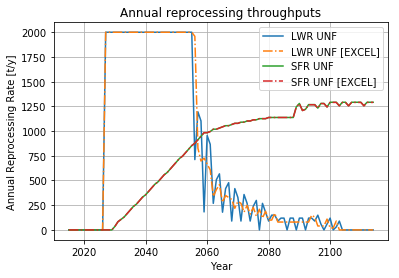
\includegraphics[scale=0.6]{./images/results_18/rep.png}
    \end{center}
        \caption{Annual reprocessing throughputs.}
    \label{fig:rep}
\end{figure}


Figure \ref{fig:tru} shows the inventory of unused \gls{TRU} recovered from \gls{UNF}.
The \Cyclus results follows the excel solutions closely. However, the difference
in core size causes \Cyclus results to be smaller, since more \gls{TRU} is used to
start up the newly deployed \glspl{SFR}. As the \glspl{SFR} \gls{UNF} is used to
create \gls{SFR} fuel, the difference is lessened.

\begin{figure}[htbp!]
	\begin{center}
		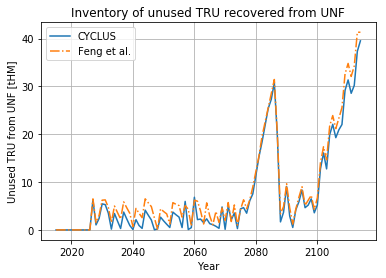
\includegraphics[scale=0.6]{./images/results_18/tru.png}
	\end{center}
        \caption{Inventory of unused \gls{TRU} recovered from \gls{UNF}.}
	\label{fig:tru}
\end{figure}


\section{Discussion}

We benchmarked \Cyclus with results from an established
verification study and saw good agreement
in a transition scenario.

Throughout this work, two major differences were identified
that led to the deviation
of \Cyclus results from that of the benchmark solution. First,
the \Cycamore reactor depletes only half of its core
when decommissioned. Second, \Cyclus, unlike other
codes examined in the benchmark (except ORION), fully resolves
discrete batches for fuel discharge.
We resolve the first discrepancy by changing one line in the source code.

This study proves \Cyclus as a capable tool for modeling
fuel cycle transition scenarios, and shows promise for
expansion and future development.


\bibliographystyle{abbrv}
\bibliography{./bibliography.bib}

\section{Appendix}

\subsection{Fresh and Used Fuel Composition}
\begin{table}[h]
	\centering
	\scalebox{0.86}{
		\begin{tabular}{|c|c|c|c|c|c|c|}
			\hline
			  Isotope 	 & 	Fresh UOX & 	Tailings & 	Spent MOX from PWR & 	Spent UOX & 	Spent MOX from SFR & 	Fresh MOX \\ \hline 
			  He4	 & 	0& 	0 & 	2.5108E-05 & 	2.0968E-07 & 	0.0004 & 	0 \\ \hline 
			  Ra226	 & 	0& 	0 & 	6.8586E-14 & 	1.1889E-14 & 	5.9399E-13 & 	0 \\ \hline 
			  Ra228	 & 	0& 	0 & 	1.0769E-19 & 	6.0516E-21 & 	1.1635E-20 & 	0 \\ \hline 
			  Pb206	 & 	0& 	0 & 	3.6378E-18 & 	7.6685E-20 & 	3.2805E-18 & 	0 \\ \hline 
			  Pb207	 & 	0& 	0 & 	1.0589E-15 & 	6.5186E-17 & 	1.4929E-15 & 	0 \\ \hline 
			  Pb208	 & 	0& 	0 & 	2.0018E-12 & 	1.2309E-13 & 	3.2098E-10 & 	0 \\ \hline 
			  Pb210	 & 	0& 	0 & 	1.1829E-19 & 	2.4968E-20 & 	1.2789E-16 & 	0 \\ \hline 
			  Th228	 & 	0& 	0 & 	4.9017E-12 & 	6.5636E-13 & 	0.0000 & 	0 \\ \hline 
			  Th229	 & 	0& 	0 & 	1.4379E-12 & 	1.7069E-13 & 	3.8020E-11 & 	0 \\ \hline 
			  Th230	 & 	0& 	0 & 	2.3998E-09 & 	0.0000 & 	4.3624E-08 & 	0 \\ \hline 
			  Th232	 & 	0& 	0 & 	8.7655E-10 & 	1.5649E-10 & 	1.7238E-10 & 	0 \\ \hline 
			  Bi209	 & 	0& 	0 & 	2.6878E-16 & 	2.5848E-17 & 	2.2881E-13 & 	0 \\ \hline 
			  Ac227	 & 	0& 	0 & 	2.4608E-14 & 	3.4567E-15 & 	6.6525E-14 & 	0 \\ \hline 
			  Pa231	 & 	0& 	0 & 	7.0696E-10 & 	2.2518E-10 & 	0.0000 & 	0 \\ \hline 
			  U232	 & 	0& 	0 & 	5.9336E-10 & 	1.3999E-10 & 	1.0759E-07 & 	0 \\ \hline 
			  U233	 & 	0& 	0.0000 & 	1.0359E-08 & 	1.3169E-09 & 	2.2135E-07 & 	0 \\ \hline 
			  U234	 & 	0.0002& 	0.0002 & 	0.0002 & 	0.0001 & 	0.0057 & 	0.0001 \\ \hline 
			  \textbf{U235}	 & 	0.0319& 	0 & 	0.0043 & 	0.0080 & 	0.0014 & 	0.0071 \\ \hline 
			  U236	 & 	0& 	0.9997 & 	0.0051 & 	0.0038 & 	0.0021 & 	0.0053 \\ \hline 
			  \textbf{U238}	 & 	0.9677& 	0 & 	0.8283 & 	0.9441 & 	0.1754 & 	0.8562 \\ \hline 
			  Np237	 & 	0& 	0 & 	0.0043 & 	0.0003 & 	0.0079 & 	0.0065 \\ \hline 
			  Pu238	 & 	0& 	0 & 	0.0060 & 	0.0001 & 	0.0497 & 	0.0032 \\ \hline 
			  \textbf{Pu239}	 & 	0& 	0 & 	0.0410 & 	0.0050 & 	0.0757 & 	0.0660 \\ \hline 
			  Pu240	 & 	0& 	0 & 	0.0283 & 	0.0022 & 	0.1493 & 	0.0312 \\ \hline 
			  \textbf{Pu241}	 & 	0& 	0 & 	0.0146 & 	0.0012 & 	0.0272 & 	0.0147 \\ \hline 
			  Pu242	 & 	0& 	0 & 	0.0098 & 	0.0004 & 	0.0768 & 	0.0091 \\ \hline 
			  Pu244	 & 	0& 	0 & 	2.1888E-07 & 	1.2459E-08 & 	5.2143E-07 & 	0 \\ \hline 
			  Am241	 & 	0& 	0 & 	0.0021 & 	2.9798E-05 & 	0.0583 & 	0 \\ \hline 
			  Am242m	 & 	0& 	0 & 	5.0357E-05 & 	3.5577E-07 & 	0.0580 & 	0 \\ \hline 
			  Am243	 & 	0& 	0 & 	0.0020 & 	7.8905E-05 & 	0.0534 & 	0 \\ \hline 
			  Cm242	 & 	0& 	0 & 	0.0002 & 	1.1579E-05 & 	0.0046 & 	0 \\ \hline 
			  Cm243	 & 	0& 	0 & 	1.2639E-05 & 	0.0000 & 	0.0004 & 	0 \\ \hline 
			  Cm244	 & 	0& 	0 & 	0.0010 & 	2.2098E-05 & 	0.0430 & 	0 \\ \hline 
			  Cm245	 & 	0& 	0 & 	0.0001 & 	1.0269E-06 & 	0.0112 & 	0 \\ \hline 
			  Cm246	 & 	0& 	0 & 	6.1406E-06 & 	9.5684E-08 & 	0.0058 & 	0 \\ \hline 
			  Cm247	 & 	0& 	0 & 	1.2059E-07 & 	8.3955E-10 & 	0.0002 & 	0 \\ \hline 
			  Cm248	 & 	0& 	0 & 	9.1585E-09 & 	4.3267E-11 & 	1.8303E-05 & 	0 \\ \hline 
			  Cm250	 & 	0& 	0 & 	3.7338E-17 & 	1.9968E-19 & 	5.1287E-12 & 	0 \\ \hline 
			  Cf249	 & 	0& 	0 & 	4.0567E-11 & 	4.3937E-14 & 	2.3787E-07 & 	0 \\ \hline 
			  Cf250	 & 	0& 	0 & 	2.9328E-11 & 	8.1175E-14 & 	0.0000 & 	0 \\ \hline 
			  Cf251	 & 	0& 	0 & 	1.4479E-11 & 	3.1608E-14 & 	8.8024E-10 & 	0 \\ \hline 
			  Cf 252	 & 	0& 	0 & 	7.5346E-12 & 	1.6679E-14 & 	1.9786E-11 & 	0 \\ \hline 
			  H3	 & 	0& 	0 & 	1.0269E-07 & 	5.7486E-08 & 	4.9486E-07 & 	0 \\ \hline 
			  C14	 & 	0& 	0 & 	3.9587E-11 & 	2.6308E-11 & 	0 & 	0 \\ \hline 
			  Kr81	 & 	0& 	0 & 	7.3446E-11 & 	2.1608E-11 & 	1.0918E-11 & 	0 \\ \hline 
			  Kr85	 & 	0& 	0 & 	2.0548E-05 & 	2.4168E-05 & 	6.7551E-05 & 	0 \\ \hline 
			  Sr90	 & 	0& 	0 & 	0.0004 & 	0.0005 & 	0.0012 & 	0 \\ \hline 
			  Tc99	 & 	0& 	0 & 	0.0011 & 	0.0007 & 	0.0042 & 	0 \\ \hline 
			  I129	 & 	0& 	0 & 	0.0003 & 	0.0001 & 	0.0011 & 	0 \\ \hline 
			  Cs134	 & 	0& 	0 & 	0.0002 & 	0.0001 & 	0.0001 & 	0 \\ \hline 
			  Cs135	 & 	0& 	0 & 	0.0009 & 	0.0003 & 	0.0077 & 	0 \\ \hline 
			  
			 
		\end{tabular}}
		\caption{Fresh and Spent Fuel Compositions}
		\label{tab:comp}
\end {table}


\end{document}
